\documentclass[dvipsnames, svgnames, x11names]{beamer}
\usetheme{mytheme2024}
\special{dvipdfmx:config z 0} %取消PDF压缩，加快速度，最终版本生成的时候最好把这句话注释掉

\title{化学反应工程}
\subtitle{第五章\ 停留时间分布与流动模型}
\author{张斌}
\institute[理工系]{河北农业大学 理工系}
\date{\the\year 年 \the\month 月}
%-----------------------------------------------------------------
\begin{document}

\maketitle


	\begin{frame}{}
        \begin{center}
            {\Huge \cbf{目 \ 录}}
        \end{center}
		\tableofcontents
		\thispagestyle{empty}
		\addtocounter{framenumber}{-1}
	\end{frame}


    \section{停留时间分布}


    \begin{frame}
        \frametitle{停留时间分布}
    
        化学反应进行的完全程度与反应物料在反应器内停留时间的长短有关，时间越长，反应进行得越完全，可见，研究反应物料在反应器内的停留时间问题具有十分重要的意义。
    
        通常所说的停留时间是指流体以进入系统时算起，到其离开系统时为止，在系统内总共经历的时间，即流体从系统的进口至出口所耗费的时间。
        \begin{itemize}
            \item 间歇反应器不存在停留时间分布问题
            \item 连续操作反应器，不同粒子停留时间是否相同？
            \begin{itemize}
                \item[\bullet] 活塞流反应器 \qquad $\surd$ 
                \item[\bullet] 连续釜式反应器 \quad $\times$ 
            \end{itemize}
        \end{itemize}
    
    \end{frame}
    
    
    \begin{frame}
        \frametitle{两种停留时间分布}
    
        \begin{itemize}
            \item 寿命分布
            
            流体粒子从进入系统起到离开系统止，在系统内停留的时间。
            \item 年龄分布
            
            对留存在系统中的流体粒子而言，从进入系统算起在系统中停留的时间。
        \end{itemize}
        \begin{figure}
            \centering
            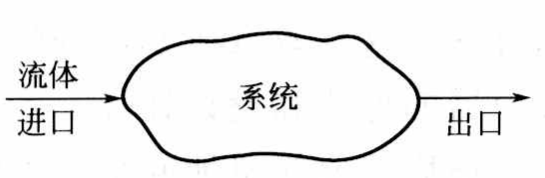
\includegraphics[width=.8\linewidth]{figures/fig5.1.png}
        \end{figure}
       
    
    \end{frame}
    
    
    \begin{frame}
        \frametitle{停留时间分布的定量描述}
    
        \begin{minipage}{0.48\linewidth}
            \begin{figure}
                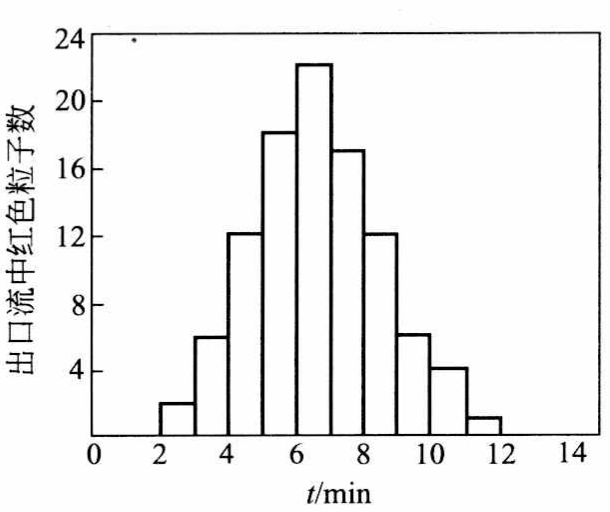
\includegraphics[width=\linewidth]{figures/fig5.2.png}
                \caption{停留时间分布直方图}
            \end{figure}
        \end{minipage}\hfill
        \begin{minipage}{0.48\linewidth}
            \begin{enumerate}
                \item 某时刻向入口加入100个红色粒子
                \item 在出口处记录不同时间间隔内流出的红色粒子数
                \item 根据观察结果作图
            \end{enumerate}
        \end{minipage}
    
    \end{frame}
    
    
    \begin{frame}
        \frametitle{停留时间分布的定量描述}
        \begin{minipage}{0.48\linewidth}
            \begin{figure}
                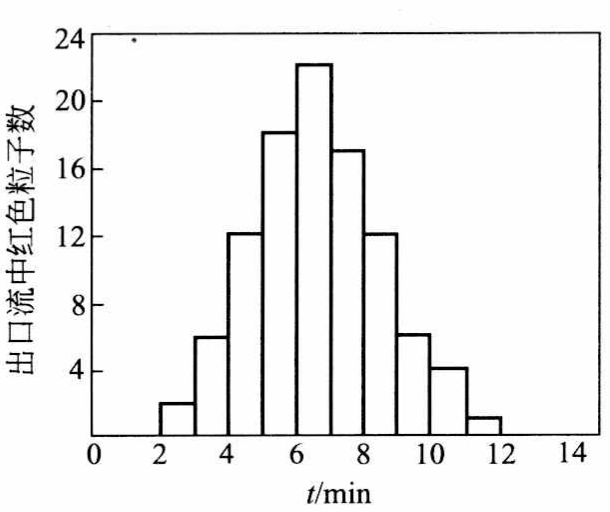
\includegraphics[width=\linewidth]{figures/fig5.2.png}
                \caption{停留时间分布直方图}
            \end{figure}
        \end{minipage}\hfill
        \begin{minipage}{0.48\linewidth}
            红色粒子由恒定流量$Q$的流体带入系统。
            
            $N_i$ 表示第 i 个时间段$\Delta t_i$流出系统的单位流体体积中红色粒子的个数。
            
            粒子的总个数 $N_\mathrm{t}=100$。
            
            各时间间隔内红色粒子所占分率之和为
            \[
                \sum_{i=0}^{\infty}\frac{QN_{i}}{N_{t}}\Delta t_{i}=\frac{1}{N_{t}}\sum_{i=0}^{\infty}QN_{i}\Delta t_{i}
            \]
            当$\Delta t_i \to 0$时，
            \[
                \frac{QN_{i}}{N_{t}} = E(t) \quad \mathrm{s^{-1}}
            \]
        \end{minipage}
    \end{frame}
    
    
    \begin{frame}
        \frametitle{停留时间分布密度函数}
    
        \begin{minipage}{0.44\linewidth}
            \begin{figure}
                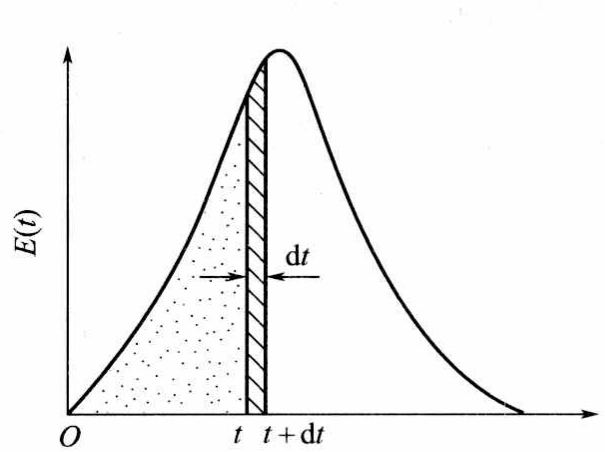
\includegraphics[width=\linewidth]{figures/fig5.3.png}
                \caption{停留时间分布密度函数}
            \end{figure}
        \end{minipage}\hfill
        \begin{minipage}{0.52\linewidth}
            \begin{enumerate}
                \item 改用红色流体作示踪剂
                \item 连续检测出口流中红色流体的浓度
                \item 观察结果将是一条连续的停留时间分布曲线
            \end{enumerate}
        \end{minipage}
    
        $E(t) \dif t$表示流体粒子在系统内的停留时间介于$t$到$t+\dif t$之间的概率。
    
        $E(t)$叫做停留时间分布密度函数，其量纲是[时间]$^{-1}$。
    
    \end{frame}
    
    
    \begin{frame}
        \frametitle{停留时间分布函数}
    
        \begin{minipage}{0.44\linewidth}
            \begin{figure}
                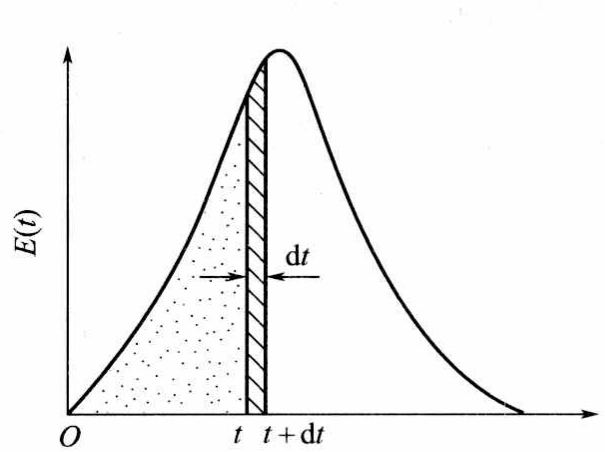
\includegraphics[width=\linewidth]{figures/fig5.3.png}
                \caption{停留时间分布密度函数}
            \end{figure}
            
        \end{minipage}\hfill
        \begin{minipage}{0.52\linewidth}
            \[
            E(t)=0 \qquad (t<0)
        \]
        \[
            E(t)\geqslant 0 \qquad (t\geqslant 0)
        \]
        \[
            \int_0^\infty E(t)\dif t =1
        \]
        \[
            \int_0^t E(t)\dif t = F(t)
        \]
        \end{minipage}
    
        $F(t)$叫做停留时间分布函数，其意义是停留时间小于$t$的流体粒子所占的分数。
    
        从概率论的角度，$F(t)$表示流体粒子的停留时间小于$t$的概率。
    
    \end{frame}
    
    
    \begin{frame}
        \frametitle{停留时间分布的定量描述}
    
        \begin{minipage}{0.46\linewidth}
            \begin{figure}
                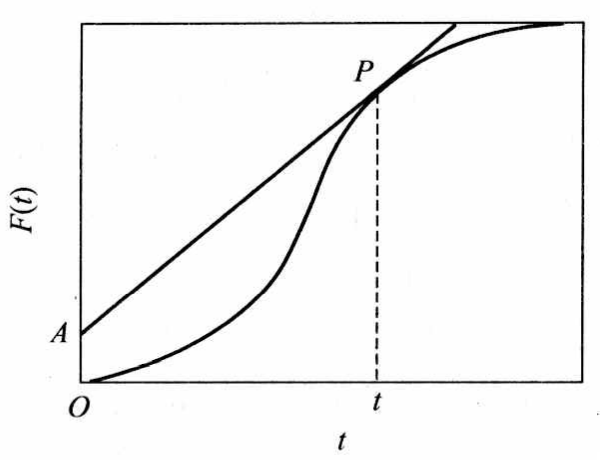
\includegraphics[width=\linewidth]{figures/fig5.4.png}
                \caption{停留时间分布函数}
            \end{figure}        
        \end{minipage}\hfill
        \begin{minipage}{0.48\linewidth}
            \begin{itemize}
                \item $F(t)$曲线是一条单调递增的线
                \item $F(t)$最大值为1，$F(\infty) =1$
                \item $F(t) =0 \qquad (t \leqslant 0)$
            \end{itemize}
    
            \[
                E(t) = \frac{\dif F(t)}{\dif t}
            \]
        \end{minipage}
    
        
    
    \end{frame}
    
    
    \begin{frame}
        \frametitle{$E(t)$和$F(t)$的关系}
        \begin{figure}[htpb]
            \centering
            \setcounter{subfigure}{0}
            \subfloat[$F(t) = \int_0^t E(t)\dif t$]{
\includegraphics[height=4.5cm]{fig5.3.png}}\quad
            \subfloat[$E(t) = \frac{\dif F(t)}{\dif t}$]{
\includegraphics[height=4.5cm]{fig5.4.png}}
        \end{figure}
        \begin{itemize}
          \item 若$E(t)$曲线已知，将其进行积分即得相应的$F(t)$值。
          \item 若$F(t)$曲线已知，在线上的一点作切线，该直线的斜率即等于相应的$E(t)$值。
        \end{itemize}
    \end{frame}
    
    
    \begin{frame}
        \frametitle{无因次停留时间}
    
        有时为了应用上方便，常常使用无因次停留时间$\theta$
        \[
            \theta = \frac{\ t\ }{\bar{t}}
        \]
        式中$\bar{t}$为平均停留时间，对于在闭式系统中流动的流体，当流体密度维持不变时，其平均停留时间等于
        \[
            \bar{t} = \frac{V_\mathrm{r}}{Q}
        \]
        如果一个流体粒子的停留时间介于区间$(t$，$t+\dif t)$内，则它的无因次停留时间也一定介于区间$(\theta$，$\theta+\dif \theta)$内，因为这所指的是同一事件。
        \[
            E(t)\dif t = E(\theta)\dif \theta 
        \]
    
    \end{frame}
    
    
    \begin{frame}
        \frametitle{停留时间分布无因次化}
    
        $E(\theta)$与$E(t)$的关系为
        \[
            E(\theta) = \bar{t} E(t)
        \]
        $F(t)$本身是一累积概率，
        \[
            F(\theta) = F(t)
        \]
        \[
            \begin{aligned}
                &\int_0^\infty E(\theta)\dif \theta =1   \\
                &\int_0^\theta E(\theta)\dif \theta = F(\theta) \\
                &E(\theta) = \frac{\dif F(\theta)}{\dif \theta}
            \end{aligned}
        \]
    
    \end{frame}


    \section{停留时间分布的实验测定}


\begin{frame}
    \frametitle{脉冲法}

    在极短的时间内、在系统入口处向流进系统的流体加入一定量的示踪剂，输入示踪剂后，立刻检测系统出口处流体中示踪剂浓度随时间的变化。
    \vspace{-4pt}
    \begin{figure}
        \centering
        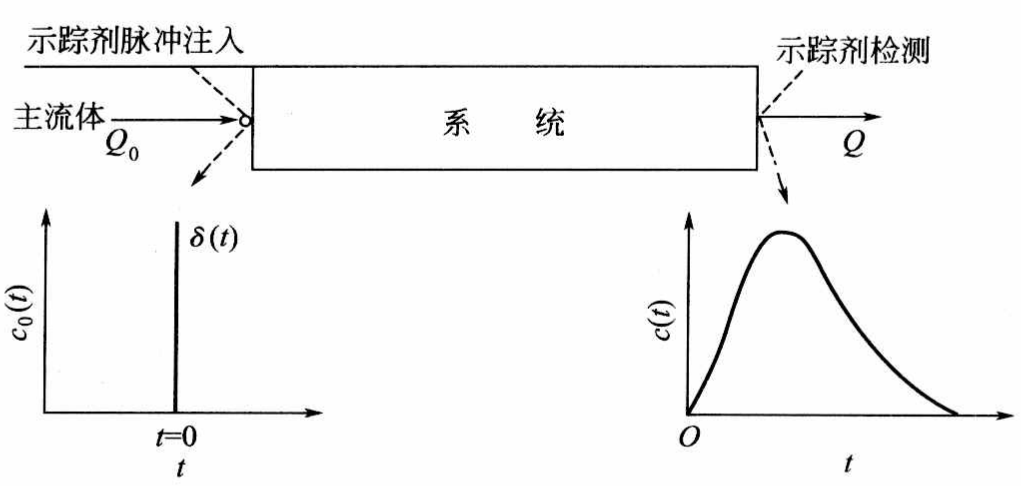
\includegraphics[width=.55\linewidth]{figures/fig5.5.png}
    \end{figure}
    \vspace{-7pt}
    \begin{blankblock}{}
        狄拉克$\delta$函数是一个广义函数，在物理学中常用其表示质点、点电荷等理想模型的密度分布，该函数在除了零以外的点取值都等于零，而其在整个定义域上的积分等于1。
    \end{blankblock}

\end{frame}
% 物理学中常常要研究一个物理量在空间或时间中分布的密度，例如质量密度、电荷密度、每单位时间传递的动量（即力）等等，但是物理学中又常用到质点、点电荷、瞬时力等抽象模型，他们不是连续分布于空间或时间中，而是集中在空间中的某一点或者时间中的某一瞬时，那么它们的密度应该如何表示呢？
% 上述表达式不规定δ函数在0点的取值，是因为这个值无法严谨地表述出来，不能笼统的定义为正无穷，并且函数取值的“大小”是由第二个积分式决定的，因此只需限定取值为零的区域即可。


\begin{frame}
    \frametitle{脉冲法}

    根据$E(t)$的定义得
    \[
        Q c(t) \mathrm{d} t=m E(t) \mathrm{d} t
    \]
    \[
        E(t)=\frac{Q c(t)}{m}
    \]
    $m$为加入示踪剂的量（mol）。

    当示踪剂的量不能准确知道时，可通过下式计算：
    \[
        m=\int_{0}^{\infty} Q_{c}(t) \mathrm{d} t
    \]
    \[
        E(t)=\frac{c(t)}{\int_{0}^{\infty} c(t) \mathrm{d} t}
    \]

\end{frame}


\begin{frame}[t]
    \frametitle{}

    \begin{example}
        流化床催化裂化装置中的再生器，其作用系用空气燃烧硅铝催化剂上的积炭使之再生。进入再生器的空气流量为\SI{0.84}{kmol.s^{-1}}现用氦气作示踪剂，采用脉冲法测定气体在再生器中的停留时间分布，氦的注入量为\SI{8.84e-3}{kmol}。试求$t=35s$时的停留时间分布密度和停留时间分布函数。
        \begin{table}[]
            \caption{再生器出口气体中氦的浓度$c$（用氦与其他气体的摩尔比表示）和时间的关系}
            \begin{tabular}{l|lllllllll}
            \hline
            $t/s$ & 0 & 9.6 & 15.1 & 20.6 & 25.3 & 30.7 & 41.8 & 46.8 & 51.8 \\ \hline
            $c \times 10^6$ & 0 & 0 & 143 & 378 & 286 & 202 & 116 & 73.5 & 57.7 \\ \hline
            \end{tabular}
            \end{table}
    \end{example}

\end{frame}


\begin{frame}
    \frametitle{阶跃法}

    \begin{itemize}
        \item 升阶法
        
        将在系统中作定常流动的流体切换为流量相同的含有示踪剂的流体
        \item 降阶法
        
        将在系统中作定常流动的含有示踪剂的流体切换为流量相同的不含示踪剂的流体
    \end{itemize}

    \begin{figure}
        \centering
        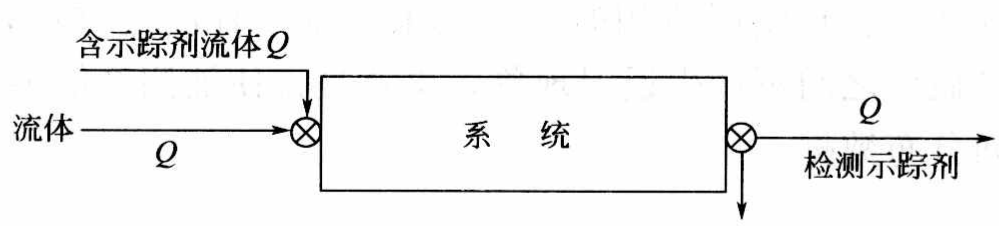
\includegraphics[width=.9\linewidth]{figures/fig5.6a.png}
    \end{figure}

\end{frame}


\begin{frame}
    \frametitle{升阶法}

    \begin{figure}
        \centering
        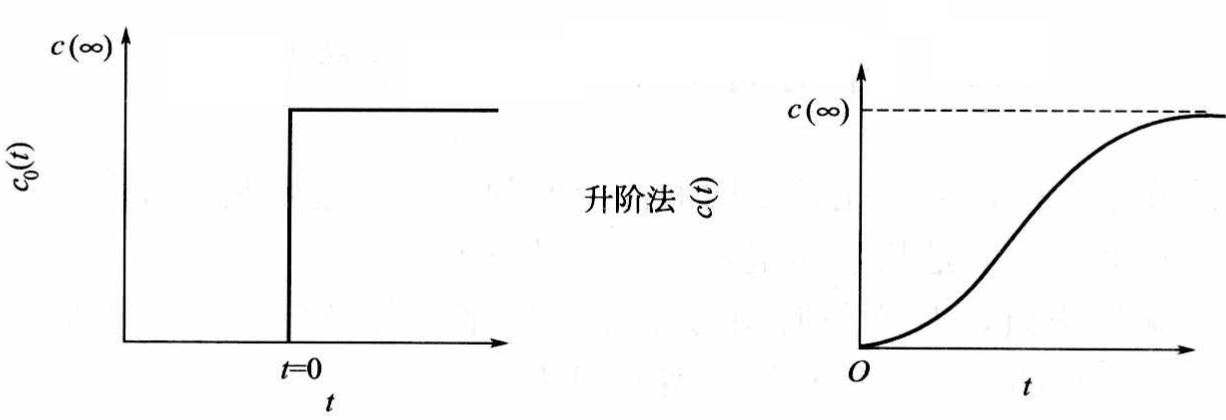
\includegraphics[width=.9\linewidth]{figures/fig5.6b.png}
    \end{figure}
    \begin{minipage}{0.48\linewidth}
        输入的阶跃函数

        $c_0(t) = 0 \qquad (t<0)$
        
        $c_0(t) = c(\infty)=\text{常数} \qquad (t\geqslant 0)$
    \end{minipage}\hfill
    \begin{minipage}{0.48\linewidth}
        \[
        F(t) = \frac{Qc(t)\dif t}{Qc(\infty)\dif t} = \frac{c(t)}{c(\infty)} = \frac{c(t)}{c(0)}
        \]
    \end{minipage}

\end{frame}


\begin{frame}
    \frametitle{降阶法}

    \begin{figure}
        \centering
        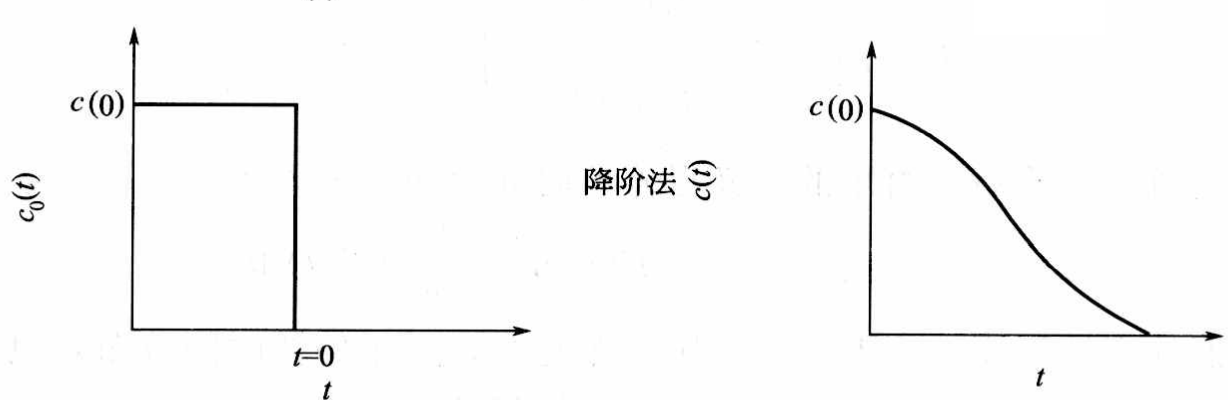
\includegraphics[width=.9\linewidth]{figures/fig5.6c.png}
    \end{figure}
    \begin{minipage}{0.48\linewidth}
        输入的阶跃函数

        $c_0(t) = c_0 =\text{常数} \qquad (t<0)$
        
        $c_0(t) = 0 \qquad (t\geqslant 0)$
    \end{minipage}\hfill
    \begin{minipage}{0.48\linewidth}
        $c(t)/c(0)$为停留时间大于$t$的物料所占的分数
        \[
        1 - F(t) = c(t)/c(0)
        \]
    \end{minipage}

\end{frame}


\begin{frame}
    \frametitle{选择示踪剂的原则}

    \begin{enumerate}
        \item 示踪剂不与主流体发生反应；
        \item 示踪剂应当易于和主流体溶为（或混为）一体，除了显著区别于主流体的某一可检测性质外，两者应具有尽可能相同的物理性质；
        \item 示踪剂浓度很低时也能够容易进行检测，这样可使示踪剂用量减少而不致影响主流体的流动；
        \item 示踪剂的浓度与要检测的物理量的关系应有较宽的线性范围，以便直接利用实验测定数据进行计算而不必再作校正和变换；
        \item 用于多相系统的示踪剂不发生从一相转移到另一相的情况，例如，气相示踪剂不能被液体所吸收，而液相示踪剂也不能挥发到气相中去；
        \item 示踪剂本身应具有或易、于转变为电信号或光信号的特点，从而能在实验中直接使用现代仪器和计算机采集数据作实时分析，以提高实验的速度和数据的精度。
    \end{enumerate}

\end{frame}


\begin{frame}
    \frametitle{脉冲法/阶跃法的比较}

    \begin{table}[]
        \caption{脉冲法/阶跃法的优缺点}
        \begin{tabular}{l|cc}
        \hline
         & 优点 & 缺点 \\ \hline
        脉冲法 & \makecell{示踪剂消耗量少 \\ 可直接求出$E(t)$} & 如何使示踪剂的输入时间缩到最短 \\ \cline{2-3} 
        阶跃法 & 容易操作 & \makecell{示踪剂用量较多 \\ 直接求出的是$F(t)$} \\ \hline
        \end{tabular}
        \end{table}
        在实际应用时，无论采用哪一种测定方法，都必须保证在示踪剂输入点与系统入口截面之间不产生返混现象，也就是说使被测系统为闭式系统，这样才可获得准确的停留时间分布数据。

\end{frame}


\section{停留时间分布的统计特征值}


% 在概率论和统计学中，数学期望（或均值，亦简称期望）是试验中每次可能结果的概率乘以其结果的总和，是最基本的数学特征之一。它反映随机变量平均取值的大小。
% 设连续性随机变量X的概率密度函数为f(x)，若积分绝对收敛，则称积分$\int_{0}^{\infty} t E(t) \mathrm{d} t$的值为随机变量的数学期望


\begin{frame}
    \frametitle{平均停留时间}
    与其他统计分布一样，为了比较不同的停留时间分布，通常是比较其统计特征值。常用的统计特征值有两个。
    \begin{enumerate}
      \item 数学期望
      \item 方差
    \end{enumerate}
    数学期望也就是均值，对停留时间分布而言即平均停留时间$\bar t$

    设连续性随机变量$x$的概率密度函数为$E(x)$，若积分绝对收敛，则数学期望为
    \[
        f(x) = \int_{-\infty}^{\infty} x E(x) \mathrm{d} x
    \]
    那么平均停留时间$\bar t$
    \[
            \bar{t}=\int_{0}^{\infty} t E(t) \mathrm{d} t=\frac{\int_{0}^{\infty} t E(t) \mathrm{d} t}{\int_{0}^{\infty} E(t) \mathrm{d} t}
    \]
\end{frame}


\begin{frame}
    \frametitle{方差}
    方差为对均值的二阶矩。对于连续型随机变量$x$，若其定义域为$(a,b)$，概率密度函数为$E(x)$，连续型随机变量$x$方差计算公式
    \[
        D(x) = \int(x-\mu)^2E(x)dx
    \]
    停留时间分布的方差为
        \[
            \sigma_{\mathrm{t}}^{2}=\mu_{2}^{\prime}=\int_{0}^{\infty}(t-\bar{t})^{2} E(t) \mathrm{d} t=\int_{0}^{\infty} t^{2} E(t) \mathrm{d} t-\bar{t}^{2} 
        \]
    方差表示对均值的离散程度，方差越大，停留时间长短不一参差不齐的程度越大，即返混越大。
\end{frame}


\begin{frame}
    \frametitle{停留时间分布的统计特征值}

    若采用无因次时间，可得无因次平均停留时间及无因次方差。
    \[
        \bar{\theta}=\int_{0}^{\infty} \theta E(\theta) \mathrm{d} \theta
    \]
    \[
        \sigma_{\theta}^{2}=\frac{\sigma_{\mathrm{t}}^{2}}{\bar{t}^{2}}=\int_{0}^{\infty} \theta^{2} E(\theta) \mathrm{d} \theta-1
    \]
    $\sigma_{\theta}^{2}$介于[0,1]之间。

    当$\sigma_{\theta}^{2} \to 0$时，返混最小；

    当$\sigma_{\theta}^{2} \to 1$时，返混最大。

\end{frame}


\begin{frame}[t]
    \frametitle{}

    \begin{example}
        用（1）脉冲法；（2）升阶法分别测得一流动系统的响应曲线$c(t)$，试推导平均停留时间$\bar{t}$及方差$\sigma_{t}^{2}$与$c(t)$的关系式。
    \end{example}
    \pause
    \begin{minipage}{0.32\linewidth}
        (1) 脉冲法
        \[
            \begin{aligned}
                \bar{t}&=\frac{\int_{0}^{\infty} t c(t) \mathrm{d} t}{\int_{0}^{\infty} c(t) \mathrm{d} t} \\
                \sigma_{\mathrm{t}}^{2}&=\frac{\int_{0}^{\infty} t^2 c(t) \mathrm{d} t}{\int_{0}^{\infty} c(t) \mathrm{d} t}-\bar{t}^{2} 
            \end{aligned}
        \]
    \end{minipage}\hfill
    \begin{minipage}{0.32\linewidth}
        (2) 升阶法
        \[
            \begin{aligned}
                \bar{t}&=\int_{0}^{T} \left[1-\frac{c(t)}{c(\infty)}\right] \mathrm{d} t \\
                \sigma_{\mathrm{t}}^{2}&=2\int_{0}^{T} \left[1-\frac{c(t)}{c(\infty)}\right] \mathrm{d} t-(\bar{t})^{2} 
            \end{aligned}
        \]
    \end{minipage}\hfill
    \begin{minipage}{0.32\linewidth}
        (3) 降阶法
        \[
            \begin{aligned}
                \bar{t}&=\int_{0}^{T} \frac{c(t)}{c(0)} \mathrm{d} t \\
                \sigma_{\mathrm{t}}^{2}&=2\int_{0}^{T} \frac{tc(t)}{c(0)} \mathrm{d} t-(\bar{t})^{2} 
            \end{aligned}
        \]
    \end{minipage}
\end{frame}


\begin{frame}[t]
    \frametitle{}
    \begin{example}
        用脉冲法测定一流动反应器的停留时间分布，得到出口流中示踪剂的浓度$c(t)$与时间$t$的关系如下
        \begin{table}
            \centering
            \begin{tabular}{cccccccccccccccc}
                \bottomrule
                $t$/min & 0 & 2 & 4 & 6 & 8 & 10 & 12 & 14 & 16 & 18 & 20 & 22 & 24 \\ \hline
                $c(t)$/(g/m$^3$) & 0 & 1 & 4 & 7 & 9 & 8 & 5 & 2 & 1.5 & 1 & 0.6 & 0.2 & 0 \\ \toprule
            \end{tabular}
        \end{table}
        试求平均停留时间及方差。
    \end{example}
\end{frame}


\section{理想反应器的停留时间分布}


\begin{frame}
    \frametitle{活塞流模型}

    活塞流模型的停留时间特征就是同时进入系统的流体粒子也同时离开系统。

    若在$t=0$时向活塞流反应器的进口以$\delta$函数的形式脉冲输入示踪剂时，则其出口流体中示踪剂的浓度也呈$\delta$函数的形式。

    \begin{minipage}{0.38\linewidth}
        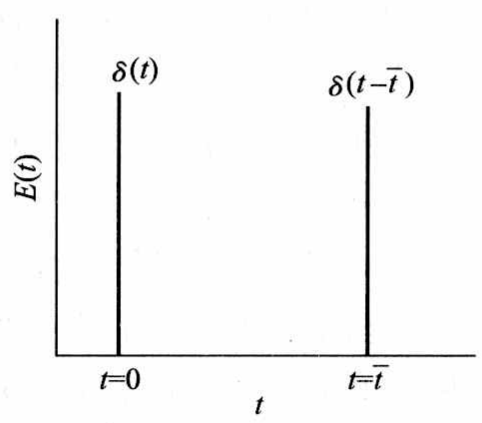
\includegraphics[width=\linewidth]{figures/fig5.7.png}
    \end{minipage}\hfill
    \begin{minipage}{0.58\linewidth}
        \[
            E(t) = \delta (t- \bar t)
        \]
        \[
            E(\theta ) = \delta (\theta- 1)
        \]
        \[
            \bar{\theta}=\int_{0}^{\infty} \theta \delta(\theta-1) \mathrm{d} \theta=\theta|_{1}=1 
        \]
        \[
            \sigma_{\theta}^{2}=\int_{0}^{\infty} \theta^{2} \delta(\theta-1) \mathrm{d} \theta-1=\theta^{2}|_{1}-1=0
        \]
    \end{minipage}

\end{frame}


\begin{frame}
    \frametitle{活塞流模型}

    \begin{minipage}{0.54\linewidth}
        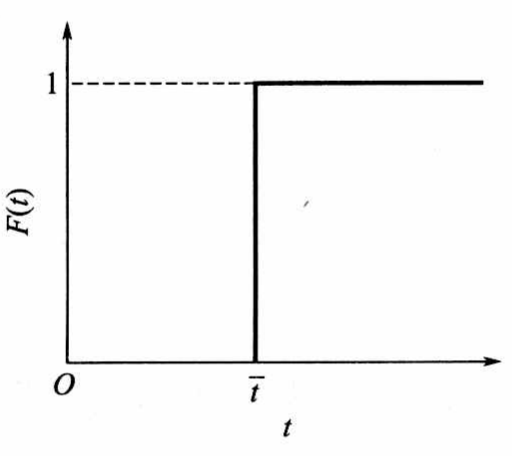
\includegraphics[width=\linewidth]{figures/fig5.8.png}
    \end{minipage}\hfill
    \begin{minipage}{0.44\linewidth}
        $F(t)=\left\{\begin{array}{ll}
            0 \quad \quad & t<\bar{t} \\
            1 \quad \quad & t \geqslant \bar{t}
            \end{array}\right.$

        \bigskip

        $F(\theta)=\left\{\begin{array}{ll}
            0 \quad \quad & \theta<1 \\
            1 \quad \quad & \theta \geqslant 1
            \end{array}\right.$
    \end{minipage}

\end{frame}


\begin{frame}
    \frametitle{全混流模型}

    设连续进入全混流反应器的流体中示踪剂的浓度为$c_0$，则单位时间内流入反应器及从反应器流出的示踪剂量分别为$Qc_0$和$Qc$。由于反应器内示踪剂的浓度均一且等于出口流中的示踪剂浓度，所以，单位时间内反应器内示踪剂的累积量为$V_r \dif c/ \dif t$，于是对反应器作示踪剂的物料衡算得
    \[
        V_r \frac{\dif c}{\dif t} = Qc_0 - Qc
    \]
    将$\tau =V_r/Q_0$代入，得
    \[
        \frac{\dif c}{\dif t} + \frac{1}{\tau}c = \frac{1}{\tau}c_0
    \]
    积分得
    \[
        \ln \frac{c_0 - c}{c_0} = - \frac{t}{\tau} \qquad \text{或} \qquad 1- \frac{c}{c_0} = e^{-t/\tau}
    \]

\end{frame}


\begin{frame}
    \frametitle{全混流模型}
    
    根据$F(t)=\frac{c(t)}{c(\infty)}=\frac{c(t)}{c(0)}$得
    \[
        F(t) = 1 - e^{-t/\tau}
    \]
    对$t$求导，得
    \[
        E(t) = \frac{1}{\tau}e^{-t/\tau}
    \]
    若采用无因次时间，则
    \[
        F(\theta) = 1 - e^{-\theta}
    \]
    对$t$求导，得
    \[
        E(\theta) = e^{-\theta}
    \]
    全混流反应器的$\bar \theta = 1$，方差$\sigma _ \theta ^2 =1$，返混程度最大。

\end{frame}


\begin{frame}
    \frametitle{全混流模型}

    \begin{figure}
        \centering
        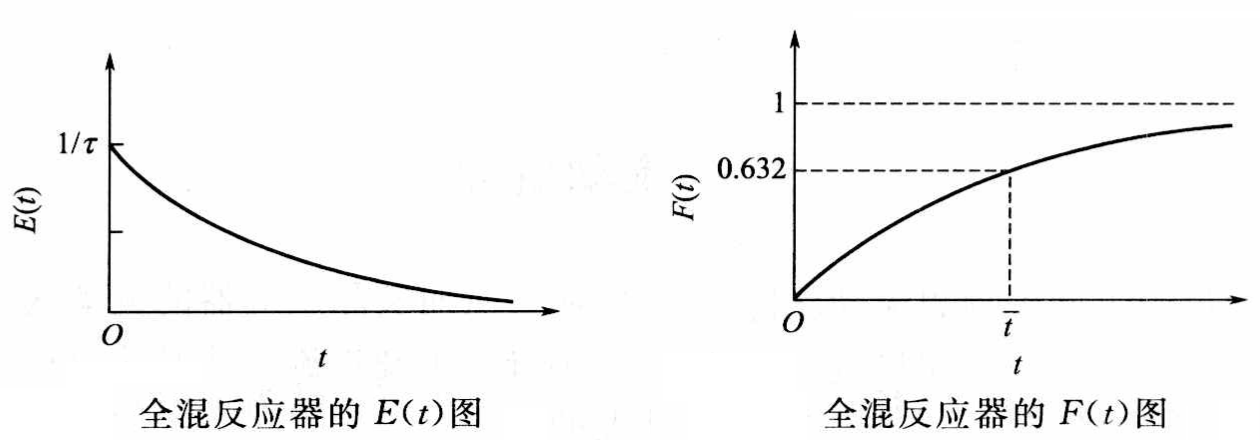
\includegraphics[width=\linewidth]{figures/fig5.9.png}
    \end{figure}
    全混流反应器，停留时间小于平均停留时间的流体粒子占全部流体的分率为$F(\bar t)=1-e^{-1}=0.632$，这部分流体的转化率小于活塞流反应器是毫无疑义的。
\end{frame}


\begin{frame}
    \frametitle{全混流模型的平均停留时间和方差}
    \[
        \begin{aligned}
            \bar{\theta}&=\int_{0}^{\infty} \theta E(\theta) \mathrm{d} \theta \\
            & = \int_{0}^{\infty} \theta e^{-\theta} \mathrm{d} \theta \\
            & = 1 \\
            \sigma_{\theta}^{2}&=\int_{0}^{\infty} \theta^{2} E(\theta) \mathrm{d} \theta-1 \\
            & = \int_{0}^{\infty} \theta^{2} e^{-\theta} \mathrm{d} \theta-1 \\
            & = 1
        \end{aligned}
    \]
\end{frame}


\begin{frame}[t]
    \frametitle{}

    \begin{example}
        设$F(\theta)$及$E(\theta)$分别为闭式流动反应器的停留时间分布函数及停留时间分布密度。

        若该反应器为活塞流反应器，下列值是多少？若该反应器为全混流反应器，下列值是多少？

        $F(1); \quad E(1); \quad F(0.8); \quad E(0.8); \quad E(1.2)$        

    \end{example}

\end{frame}


\section{非理想流动现象}


\begin{frame}
    \frametitle{非理想流动现象}

    实际反应器流动状况偏离理想流动状况的原因可归结为下列几个方面：
    \begin{enumerate}
        \item 滞流区的存在
        \item 存在沟流与短路
        \item 循环流
        \item 流体流速分布不均匀
        \item 扩散
    \end{enumerate}

\end{frame}


\section{非理想流动模型}


\begin{frame}
    \frametitle{非理想流动模型}

    \begin{enumerate}
        \item 离析流模型
        
        假如反应器内的流体粒子之间不存在任何形式的物质交换，那么流体粒子就像一个有边界的个体，从反应器的进口向出口运动，这样的流动叫做离析流。
        \item 多釜串联模型
        
        用N个全混釜串联来模拟一个实际的反应器。
        \item 轴向扩散模型
        
        由于分子扩散、涡流扩散以及流速分布的不均匀等原因，而使流动状况偏离理想流动时，可用轴向扩散模型来模拟，这对于管式反应器尤为合适。
    \end{enumerate}

\end{frame}


\begin{frame}
    \frametitle{离析流模型}

    \begin{minipage}{0.58\linewidth}
        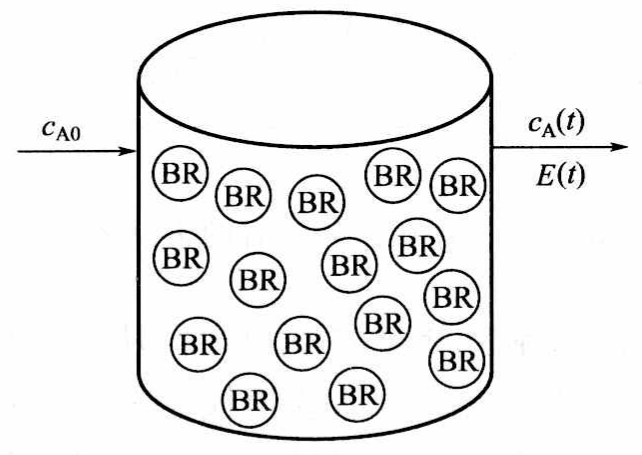
\includegraphics[width=\linewidth]{figures/fig5.16.png}
    \end{minipage}\hfill
    \begin{minipage}{0.38\linewidth}
        \begin{itemize}
            \item 假定流体粒子之间不发生微观混合
            \item BR可看作由反应物粒子群构成的间歇反应器
            \item 每个间歇反应器的反应时间取决于它们在连续流动反应器中的停留时间
        \end{itemize}
    \end{minipage}

\end{frame}


\begin{frame}
    \frametitle{离析流模型}

    根据反应器的停留时间分布知，停留时间在$t$到$t+\dif t$间的流体粒子所占的分率为$E(t)\dif t$，则这部分流体对反应器出口流体中A的浓度$\bar c_\mathrm{A}$的贡献应为$c_\mathrm{A}(t)E(t)\dif t$，将所有这些贡献相加即得反应器出口处A的平均浓度$\bar c_\mathrm{A}$，即
    \[
        \bar c_\mathrm{A} = \int_0^\infty c_\mathrm{A}(t)E(t)\dif t
    \]
    根据$c_\mathrm{A} = c_\mathrm{A0}(1 - X_\mathrm{A})$，上式可改写成
    \[
        1 - \bar X_\mathrm{A} = \int_0^\infty [1 - X_\mathrm{A}(t)]E(t)\dif t = \int_0^\infty E(t)\dif t - \int_0^\infty X_\mathrm{A}(t)E(t)\dif t
    \]
    所以
    \[
        \bar X_\mathrm{A} = \int_0^\infty X_\mathrm{A}(t)E(t)\dif t
    \]
    使用时要注意积分上限的使用（应为完全反应时间）。

\end{frame}


\begin{frame}[t]
    \frametitle{}

    \begin{example}
        等温下在反应体积为\SI{4.55}{m^3}的流动反应器中进行液相反应
        \[
            \ch{2 A -> R + P}
        \]
        该反应为二级反应，反应温度下反应速率常数$k =$\SI{2.4e-3}{m^3.mol^{-1}.min^{-1}}。进料流量为\SI{0.53}{m^3.min^{-1}}，A的浓度等于\SI{1.6}{kmol.m^{-3}}。该反应器的停留时间分布如下表所示。试计算反应器出口处A的转化率：（1）用离析流模型；（2）用活塞流模型。
        \begin{table}[]            
            \begin{tabular}{cccccccccccccc}
            \hline
            $t/\mathrm{min}$ & 0 & 2 & 4 & 6 & 8 & 10 & 12 & 14 & 16 & 18 & 20 & 22 & 24 \\ \hline
            $c /\mathrm{(g/m^3)}$ & 0 & 1 & 4 & 7 & 9 & 8 & 5 & 2 & 1.5 & 1 & 0.6 & 0.2 & 0 \\ \hline
            \end{tabular}
            \end{table}
    \end{example}

\end{frame}


\begin{frame}
    \frametitle{多釜串联模型}

    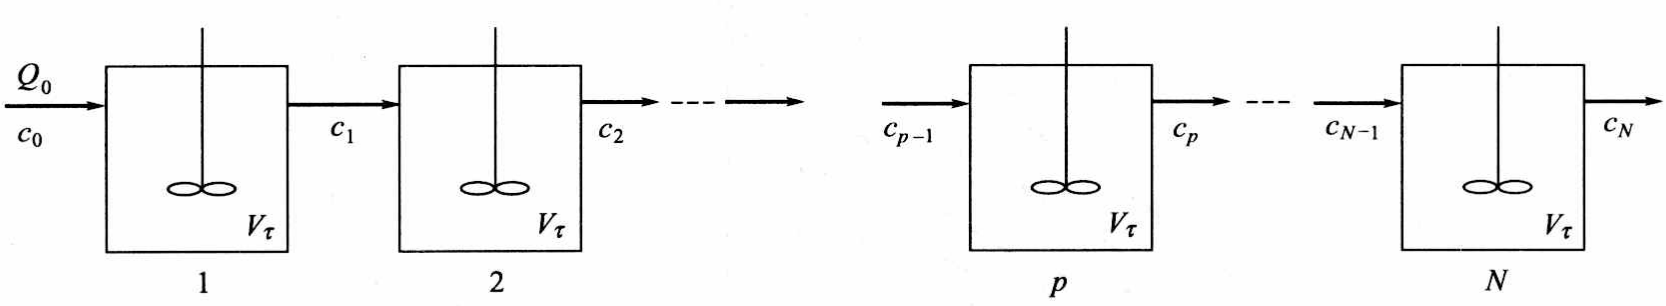
\includegraphics[width=\linewidth]{figures/fig5.17.png}

    可以用$N$个全混釜串联来模拟一个实际的反应器。$N$为模型参数。
    \begin{itemize}
        \item $N=1$时为全混流；
        \item $N=\infty$则为活塞流。
    \end{itemize}
    $N$的取值不同反映了实际反应器的不同返混程度，其具体数值由停留时间分布确定。

    为此，首先求定多釜串联时的停留时间分布。

\end{frame}


\begin{frame}
    \frametitle{多釜串联模型}

    对第$p$釜作示踪剂的物料衡算得
    \[
        Q c_{p-1}(t)-Q c_{p}(t)=V_{\mathrm{r}} \frac{\mathrm{d} c_{\mathrm{p}}(t)}{\mathrm{d} t}
    \]
    \[
        \text{或} \qquad \frac{\mathrm{d} c_{p}(t)}{\mathrm{d} t}=\frac{1}{\tau}\left[c_{p-1}(t)-c_{p}(t)\right]  \qquad
    \]
    若示踪剂呈阶跃输入，且浓度为$c_0$，则上式的初始条件为$t=0 \quad c_{p}(0)=0 \quad(p=1,2, \cdots, N)$。

    当$p=1$时，
    \[
        \frac{\mathrm{d} c_{1}(t)}{\mathrm{d} t}=\frac{1}{\tau}\left[c_{0}(t)-c_{1}(t)\right]
    \]
    此即第1釜的物料衡算式，其解为
    \[
        c_{1}(t)=c_{0}\left(1-\mathrm{e}^{-t / \tau}\right)
    \]

\end{frame}


\begin{frame}
    \frametitle{多釜串联模型}

    对于第2釜
    \[
        \frac{\mathrm{d} c_{2}(t)}{\mathrm{d} t}=\frac{1}{\tau}\left[c_{1}(t)-c_{2}(t)\right]
    \]
    将$c_{1}(t)=c_{0}\left(1-\mathrm{e}^{-t / \tau}\right)$代入，解得
    \[
        \frac{c_{2}(t)}{c_{0}}=1-\left(1+\frac{t}{\tau}\right) \mathrm{e}^{-t / \tau}
    \]
    依次对其他各釜求解，可得第N个釜的结果为
    \[
        F(t)=\frac{c_{N}(t)}{c_{0}}=1-\mathrm{e}^{-t / \tau} \sum_{p=1}^{N} \frac{(t / \tau)^{p-1}}{(p-1) !} 
    \]
    此即多釜串联系统的停留时间分布函数式。

\end{frame}


\begin{frame}
    \frametitle{多釜串联模型}

    若以系统的总平均停留时间$\tau_t = N\tau$代入，得
    \[
        F(t)=1-\mathrm{e}^{-N t / \tau_{t}} \sum_{p=1}^{N} \frac{\left(N t / \tau_{\mathrm{t}}\right)^{p-1}}{(p-1) !}
    \]
    也可以写成无因次形式
    \[
        F(\theta)=1-\mathrm{e}^{-N \theta} \sum_{p=1}^{N} \frac{(N \theta)^{p-1}}{(p-1) !}
    \]
    这里$\theta = t / \tau_{t}$，即根据系统的总平均停留时间来定义，而不是每釜的平均停留时间。

\end{frame}


\begin{frame}
    \frametitle{多釜串联模型}

    \begin{figure}        
        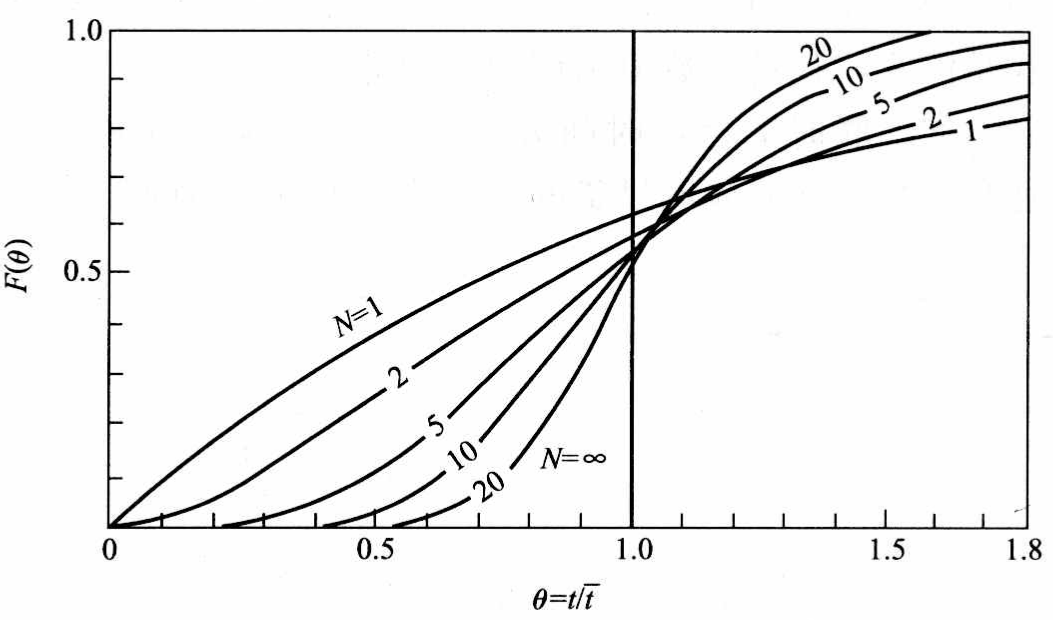
\includegraphics[width=.67\linewidth]{figures/fig5.18.png}
        \caption{多釜串联模型的$F(\theta)$图}
    \end{figure}    

\end{frame}


\begin{frame}
    \frametitle{多釜串联模型}

    将式$F(\theta)$对$\theta$求导，可得多釜串联模型的停留时间分布密度
    \[
        E(\theta)=\frac{N^{N}}{(N-1) !} \theta^{N-1} \mathrm{e}^{-N \theta}
    \]
    多釜串联模型的平均停留时间为
    \[
        \bar{\theta}=\int_{0}^{\infty} \frac{N^{N} \theta^{N} \mathrm{e}^{-N \theta}}{(N-1) !} \mathrm{d} \theta=1
    \]
    方差为
    \[
        \sigma_{\theta}^{2}=\int_{0}^{\infty} \frac{N^{N} \theta^{N+1} \mathrm{e}^{-N \theta}}{(N-1) !} \mathrm{d} \theta-1 =\frac{N+1}{N}-1=\frac{1}{N}
    \]
    当$N=1$时，$\sigma_{\theta}^{2}=1$，与全混流模型一致；而当$N=\infty$时，$\sigma_{\theta}^{2}=0$，与活塞流模型相一致。当N为任何正数时，其方差应介于0与1之间。

\end{frame}


\begin{frame}
    \frametitle{多釜串联模型}

    \begin{minipage}{0.52\linewidth}
        \begin{figure}        
            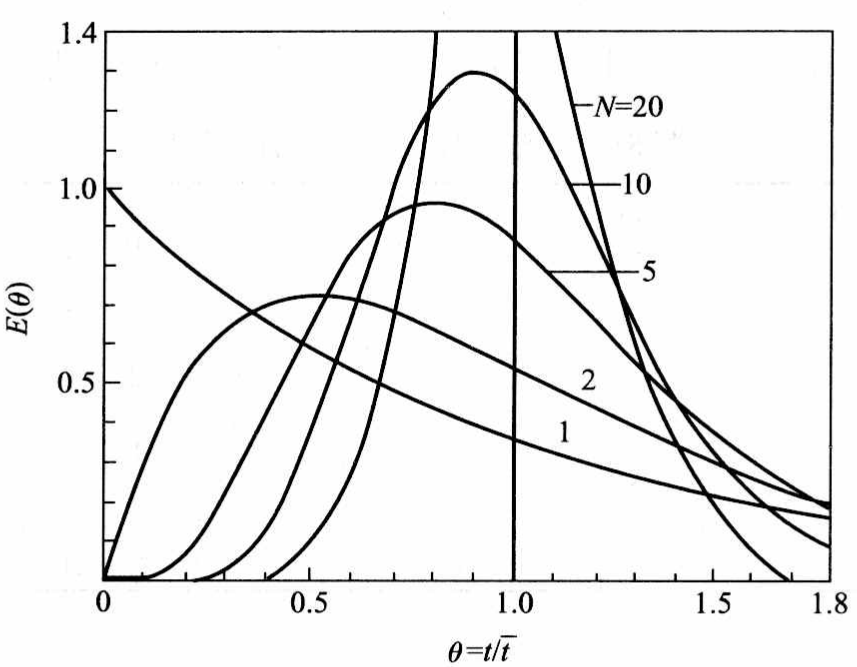
\includegraphics[width=\linewidth]{figures/fig5.19.png}
            \caption{多釜串联模型的$E(\theta)$图}
        \end{figure} 
    \end{minipage}\hfill
    \begin{minipage}{0.46\linewidth}
        \begin{itemize}
            \item $N$增加，停留时间分布变窄
        \end{itemize}
        \bigskip
        应用多釜串联模型来模拟一个实际反应器的流动状况时，首先要测定该反应器的停留时间分布，然后求出该分布的方差，将其代入$\sigma_{\theta}^{2}=\frac{1}{N}$便可算出模型参数N。
        \bigskip

        $N$为非整数？        
        \begin{itemize}
            \item 四舍五入
            \item 将小数部分视作小釜
        \end{itemize}
    \end{minipage}
     
\end{frame}


\begin{frame}[t]
    \frametitle{}
    \begin{example}
        以苯甲酸为示踪剂 ， 用脉冲法测定一反应体积为\SI{1735}{cm^3}的液相反应器的停留时间分布 。 液体流量为\SI{40.2}{cm^3/min}， 示踪剂用量4.95 g。不同时刻下出口液体中示踪物的浓度 $c(t)$ 如下表所示 。 若用多釜串联模型来模拟该反应器 ， 试求模型参数$N$。
        \begin{table}
            \centering
            \begin{tabular}{cc|cc|cc|cc}
                \bottomrule
                $t$/min & $c(t)\times 10^3$/(g/cm$^3$) & $t$ & $c(t)\times 10^3$ & $t$ & $c(t)\times 10^3$ & $t$ & $c(t)\times 10^3$   \\ \hline
                10 & 0     & 40 & 3.520 & 65 & 0.910 & 90 & 0.131  \\ 
                15 & 0.113 & 45 & 2.840 & 70 & 0.619 & 95 & 0.094  \\ 
                20 & 0.863 & 50 & 2.270 & 75 & 0.413 & 100 & 0.075  \\ 
                25 & 2.210 & 55 & 1.735 & 80 & 0.300 & 105 & 0.001  \\ 
                30 & 3.340 & 60 & 1.276 & 85 & 0.207 & 110 & 0  \\ 
                35 & 3.720 &  &  &  &  &  &  \\ \toprule
            \end{tabular}
        \end{table}
        \vspace{-5pt}
    \end{example}
\end{frame}


\begin{frame}
    \frametitle{轴向扩散模型}

    由于分子扩散、涡流扩散以及流速分布不均匀等原因，而使流动状况偏离理想流动时，可用轴向扩散模型来模拟，这对管式反应器尤为合适。该模型假定：
    \begin{enumerate}
        \item 流体以恒定的流速$u$通过系统；
        \item 垂直于流体运动方向的横截面上径向浓度分布均一，即径向混合达最大；
        \item 由于湍流混合、分子扩散以及流速分布等传递机理而产生的扩散，仅发生在流动方向（即轴向），并以轴向扩散系数$Da$表示这些因素的综合作用，且用费克定律加以描述。
    \end{enumerate}
    由于返混是逆着主流体流动方向进行，所以\highlight{扩散通量}(单位时间内通过垂直于扩散方向的单位截面积的扩散物质流量)
    \[
        J = - Da \frac{\partial c}{\partial Z}
    \]
    同时假定在同一反应器内轴向扩散系数不随时间及位置而变，其数值大小与反应器的结构、操作条件及流体性质有关。

\end{frame}


\begin{frame}
    \frametitle{轴向扩散模型}

    根据上述假设，可建立轴向扩散模型的数学模型方程。
    \begin{figure}
        \centering
        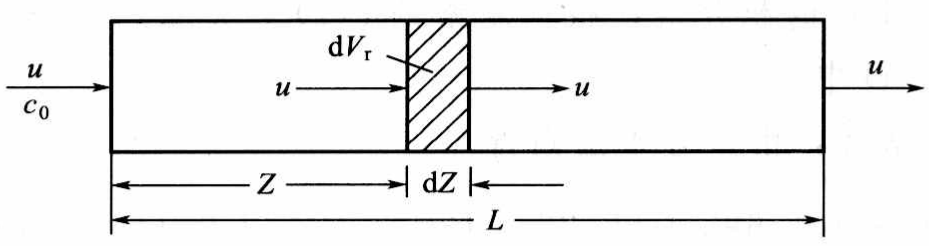
\includegraphics[width=\linewidth]{figures/fig5.20.png}
    \end{figure}
    取微元体积$\dif V_\mathrm{r}$作控制体积，对微元体积作示踪剂的物料衡算即得模型方程。

    若其横截面积为$A_\mathrm{r}$，则$\dif V_\mathrm{r} = A_\mathrm{r} \dif Z$。

\end{frame}


\begin{frame}
    \frametitle{轴向扩散模型}

    输入应包括两项，一是通过对流；另一是通过扩散。同样输出也应包括两项。
    \[
        \red{\text{输入}} = \magenta{\text{输出}} + \cyan{\text{累积}}
    \]
    \[
        \red{u A_{\mathrm{r}} c+D a A_{\mathrm{r}} \frac{\partial}{\partial Z}\left(c+\frac{\partial c}{\partial Z} \mathrm{~d} Z\right)} = \magenta{u A_{\mathrm{r}}\left(c+\frac{\partial c}{\partial Z} \mathrm{~d} Z\right)+D a A_{\mathrm{r}} \frac{\partial c}{\partial Z}
        } + \cyan{\frac{\partial c}{\partial t} A_{\mathrm{r}} \mathrm{d} Z}
    \]
    整理后，得
    \[
        \frac{\partial c}{\partial t}=D a \frac{\partial^{2} c}{\partial Z^{2}}-u \frac{\partial c}{\partial Z}
    \]
    此即轴向扩散模型方程。这里共有两个自变量，一是时间自变量$t$，另一为空间自变量，即轴向距离$Z$，所以模型方程为一偏微分方程。

    轴向扩散模型实质上是活塞流模型再迭加一扩散项，即上式右边第一项。通过此项反映系统内返混的大小。若$Da=0$，则化为活塞流模型方程
    \[
        \frac{\partial c}{\partial t}=-u \frac{\partial c}{\partial Z}
    \]
    \vspace{-10pt}
\end{frame}


\begin{frame}
    \frametitle{轴向扩散模型}

    通常将轴向扩散模型方程化为无量纲形式，这样使用起来比较方便。为此，引入下列各无因次量
    \[
        \theta=\frac{t u}{L_{\mathrm{r}}} \qquad \psi =\frac{c}{c_{0}} \qquad \zeta=\frac{Z}{L_{\mathrm{r}}} \qquad P e=\frac{u L_{\mathrm{r}}}{D a}
    \]
    轴向扩散模型无量纲方程为
    \[
        \frac{\partial \psi}{\partial \theta}=\frac{1}{P e} \frac{\partial^{2} \psi}{\partial \zeta^{2}}-\frac{\partial \psi}{\partial \zeta}
    \]
    $Pe$为贝克来数，其物理意义为
    \[
        P e=\frac{u L_{\mathrm{r}}}{D a}=\frac{\text { 对流传递速率 }}{\text { 扩散传递速率 }}
    \]
    贝克来数反映了返混的程度。$Pe$越大，返混程度越小。

\end{frame}


\begin{frame}
    \frametitle{轴向扩散模型}

    闭式系统，示踪剂以阶跃方式输入时，
    \[
        F(\theta)=1-\mathrm{e}^{P e / 2} \sum_{n=1}^{\infty} \frac{8 \omega_{\mathrm{n}} \sin \omega_{\mathrm{n}} \exp \left[-\left(P e^{2}+4 \omega_{\mathrm{n}}\right) \theta / 4 P e\right]}{P e^{2}+4 P e+4 \omega_{\mathrm{n}}^{2}}
    \]
    式中，$\omega_{\mathrm{n}}$为下列方程的正根
    \[
        \tan \omega_{\mathrm{n}}=\frac{4 \omega_{\mathrm{n}} P e}{4 \omega_{\mathrm{n}}^{2}-P e^{2}}
    \]
    \[
        E(\theta)=\mathrm{e}^{P e / 2} \sum_{n=1}^{\infty} \frac{(-1)^{\mathrm{n}+1} 8 \omega_{\mathrm{n}}^{2} \exp \left[-\left(P e^{2}+4 \omega_{\mathrm{n}}^{2}\right) \theta / 4 P e\right]}{P e^{2}+4 P e+4 \omega_{\mathrm{n}}^{2}}
    \]
    

\end{frame}


\begin{frame}
    \frametitle{轴向扩散模型}

    \begin{figure}
        \centering
        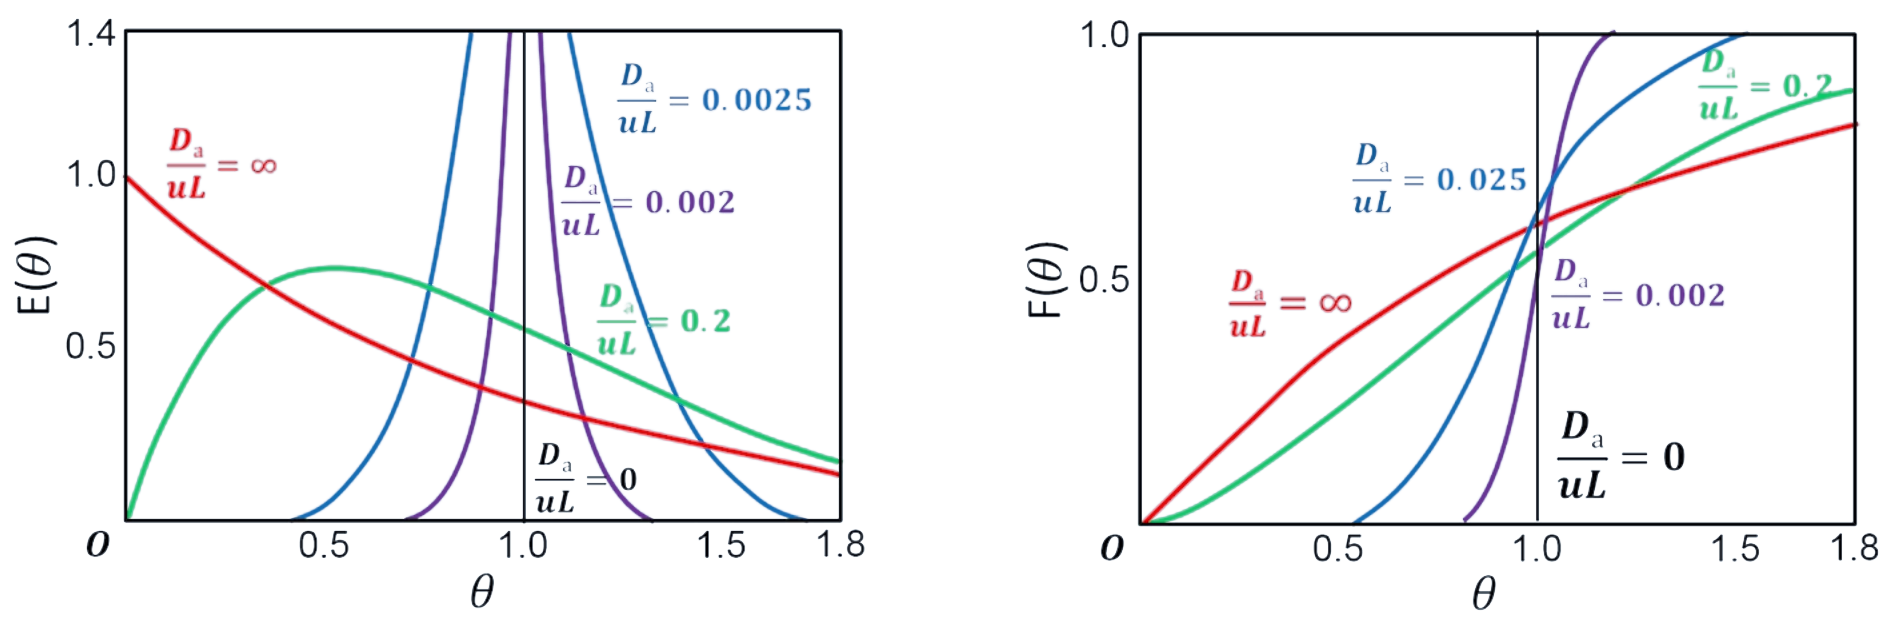
\includegraphics[width=\linewidth]{figures/fig5.21.png}
    \end{figure}
    随着模型参数$Pe$的倒数的减小，停留时间分布变窄。
    \begin{itemize}
        \item 当$Pe \to 0$时，属于全混流情况。
        \item 当$Pe \to \infty$时，属于活塞流情况
    \end{itemize}

\end{frame}


\begin{frame}
    \frametitle{轴向扩散模型}

    平均停留时间与方差为
    \[
        \bar \theta = 1
    \]
    \[
        \sigma_{\theta}^{2}=\frac{2}{P e}-\frac{2}{P e^{2}}(1-\mathrm{e}^{-P e})
    \]
    如果实际系统的停留时间分布已知，则可求出该分布的方差，代入上式试差即可求出模型参数。

    设计反应器时，停留时间分布未知，这可根据有关关联式来估算$Pe$。例如，对于空管反应器
    \[
        \frac{1}{Pe} = \frac{1}{Sc \cdot Re} + \frac{Re \cdot Sc}{192}
    \]
    若为湍流，则用
    \[
        Pe = Re^{0.125}
    \]

\end{frame}


\begin{frame}[t]
    \frametitle{}
    \begin{example}
        以苯甲酸为示踪剂 ， 用脉冲法测定一反应体积为\SI{1735}{cm^3}的液相反应器的停留时间分布 。 液体流量为\SI{40.2}{cm^3/min}， 示踪剂用量4.95 g。不同时刻下出口液体中示踪物的浓度 $c(t)$ 如下表所示 。 用轴向扩散模型来模拟该反应器 ， 试求模型参数$Pe$。
        \begin{table}
            \centering
            \begin{tabular}{cc|cc|cc|cc}
                \bottomrule
                $t$/min & $c(t)\times 10^3$/(g/cm$^3$) & $t$ & $c(t)\times 10^3$ & $t$ & $c(t)\times 10^3$ & $t$ & $c(t)\times 10^3$   \\ \hline
                10 & 0     & 40 & 3.520 & 65 & 0.910 & 90 & 0.131  \\ 
                15 & 0.113 & 45 & 2.840 & 70 & 0.619 & 95 & 0.094  \\ 
                20 & 0.863 & 50 & 2.270 & 75 & 0.413 & 100 & 0.075  \\ 
                25 & 2.210 & 55 & 1.735 & 80 & 0.300 & 105 & 0.001  \\ 
                30 & 3.340 & 60 & 1.276 & 85 & 0.207 & 110 & 0  \\ 
                35 & 3.720 &  &  &  &  &  &  \\ \toprule
            \end{tabular}
        \end{table}
        \vspace{-5pt}
    \end{example}
\end{frame}


\section{非理想反应器的计算}


\begin{frame}
    \frametitle{轴向扩散模型的计算}

    以一级反应为例，对关键组分A做物料衡算，输入 - 输出 - 消耗 = 0
    \[
        D_{\mathrm{a}} \frac{\mathrm{d}^{2} c_{\mathrm{A}}}{\mathrm{d} Z^{2}}-u \frac{\mathrm{d} c_{\mathrm{A}}}{\mathrm{d} Z}-k c_{\mathrm{A}}=0
    \]
    
    \[
       \text{结合边界条件} \qquad \qquad \qquad  Z=0, u c_{\mathrm{A} 0}=u c_{\mathrm{A}}-\left.D_{\mathrm{a}} \frac{\mathrm{d} c_{\mathrm{A}}}{\mathrm{d} Z}\right|_{0^{+}} \qquad \qquad \qquad \qquad \quad
    \]
    \[
        Z=L_{\mathrm{r}},\left.\frac{\mathrm{d} c_{\mathrm{A}}}{\mathrm{d} Z}\right|_{L_{\mathrm{r}}^{-}}=0
    \]
    解析求解得
    \[
        \frac{c_{\mathrm{A}}}{c_{\mathrm{A} 0}}=\frac{4 \alpha}{(1+\alpha)^{2} \exp \left[-\frac{P e}{2}(1-\alpha)\right]-(1-\alpha)^{2} \exp \left[-\frac{P e}{2}(1+\alpha)\right]}
    \]
    \[
        \text{式中} \qquad \alpha=(1+4 k \tau / P e)^{1 / 2}
    \]

\end{frame}


\begin{frame}
    \frametitle{轴向扩散模型的计算}

    当$Pe \to \infty$时，$\alpha \to 1$，因此可将$\alpha$展开成
    \[
        \alpha=1+\frac{1}{2}\left(\frac{4 k \tau}{P e}\right)-\frac{1}{8}\left(\frac{4 k \tau}{P e}\right)^{2}+\cdots
    \]
    代回，得
    \[
        c_{\mathrm{A}} / c_{\mathrm{A} 0}=\exp (-k \tau)
    \]
    当$Pe \to 0$时，
    \[
        \frac{c_{\mathrm{A}}}{c_{\mathrm{A} 0}}=\frac{4 \alpha}{(1+\alpha)^{2}\left(1-\frac{P e}{2}+\alpha \frac{P e}{2}\right)-(1-\alpha)^{2}\left(1-\frac{P e}{2}-\alpha \frac{P e}{2}\right)}
    \]
    \[
        =\frac{4 \alpha}{4 \alpha-\alpha P e+\alpha^{3} P e}=\frac{1}{1+k \tau} \qquad \qquad \qquad \qquad
    \]
    这与连续釜式反应器进行一级反应时的计算式一样。

\end{frame}


\begin{frame}
    \frametitle{轴向扩散模型，一级反应}
    \begin{minipage}{0.38\linewidth}
        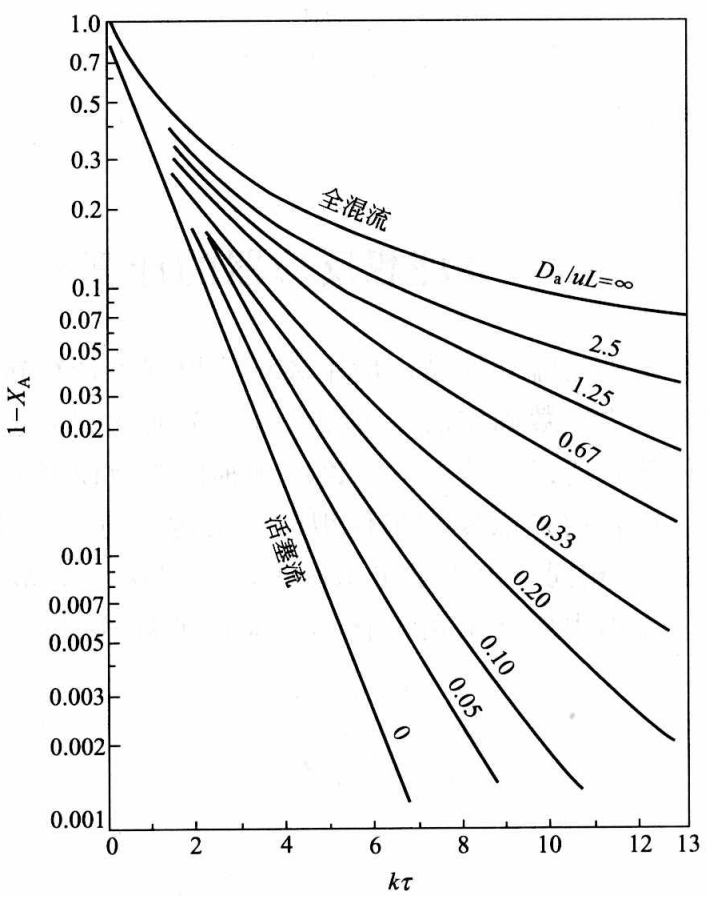
\includegraphics[width=\linewidth]{figures/fig5.23.png}
    \end{minipage}\hfill
    \begin{minipage}{0.6\linewidth}
        \begin{itemize}
            \item 具有闭式边界条件的轴向扩散模型，根据模型参数$Pe$的取值不同，可以体现从活塞流到全混流之间的任何返混情况。
            \item 实际反应器的转化率随$Pe$倒数的减小而增加。
            \item 空时越大，流动状况偏离理想流动的影响也越大。
        \end{itemize}
    \end{minipage}   

\end{frame}


\begin{frame}
    \frametitle{轴向扩散模型，二级反应}
    \begin{minipage}{0.72\linewidth}
        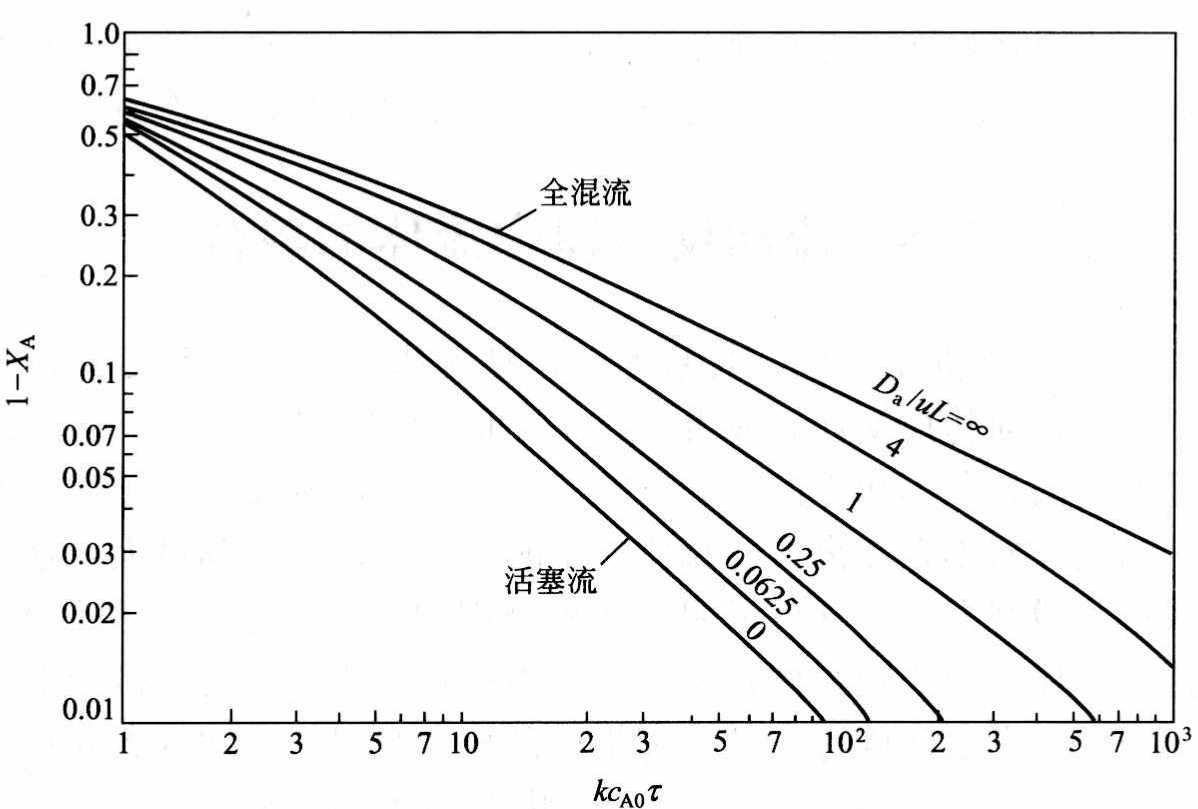
\includegraphics[width=\linewidth]{figures/fig5.24.png}
    \end{minipage}
    \begin{minipage}{0.264\linewidth}
        \begin{itemize}
            \item 在其他条件相同的情况下，二级反应的转化率受返混的影响比一级反应大。
            \item 一般而言，反应级数越高，返混对反应结果的影响越大。
        \end{itemize}
    \end{minipage}   

\end{frame}


\section{流动反应器中流体的混合}


\begin{frame}
    \frametitle{流动反应器中流体的混合}

    离析流模型，其基本假定是流体粒子从进入反应器起到离开反应器止，粒子之间不发生任何物质交换，或者说粒子之间不产生混合，这种状态称为完全离析，即各个粒子都是孤立的，各不相干的。如果粒子之间发生混合又是分子尺度的，则这种混合称为微观混合。当反应器不存在离析的流体粒子时，微观混合达到最大，这种混合状态称为完全微观混合或最大微观混合。介乎两者之间则称为部分离析或部分微观混合，即两者并存。
    \begin{itemize}
        \item 完全离析(宏观流体)    
        \item 完全微观混合(微观流体)
        \item 部分微观混合
    \end{itemize}

\end{frame}


\begin{frame}
    \frametitle{流动反应器中流体的混合}

    混合状态的不同，将对化学反应产生不同的影响。设浓度分别为$c_\mathrm{A1}$和$c_\mathrm{A2}$而体积相等的两个流体粒
子，在其中进行$\alpha$级不可逆反应。
    \begin{itemize}
        \item 完全离析
        
        \[
            \langle r_\mathrm{A}\rangle  = \frac{1}{2}(r_\mathrm{A1} + r_\mathrm{A2}) = \frac{k}{2}(c_\mathrm{A1}^{\alpha} + c_\mathrm{A2}^{\alpha})
        \]
        \item 完全微观混合
        
        \[
            \langle r_\mathrm{A}' \rangle  = k[(c_\mathrm{A1} + c_\mathrm{A2})/2]^{\alpha}
        \]
    \end{itemize}
    这就说明了微观混合程度不同将会对化学反应的速率发生影响。
    
    $\langle r_\mathrm{A}\rangle$与$\langle r_\mathrm{A}' \rangle$的大小与$\alpha$值有关。

\end{frame}


\begin{frame}
    \frametitle{流动反应器中流体的混合}

    \begin{minipage}{0.48\linewidth}
        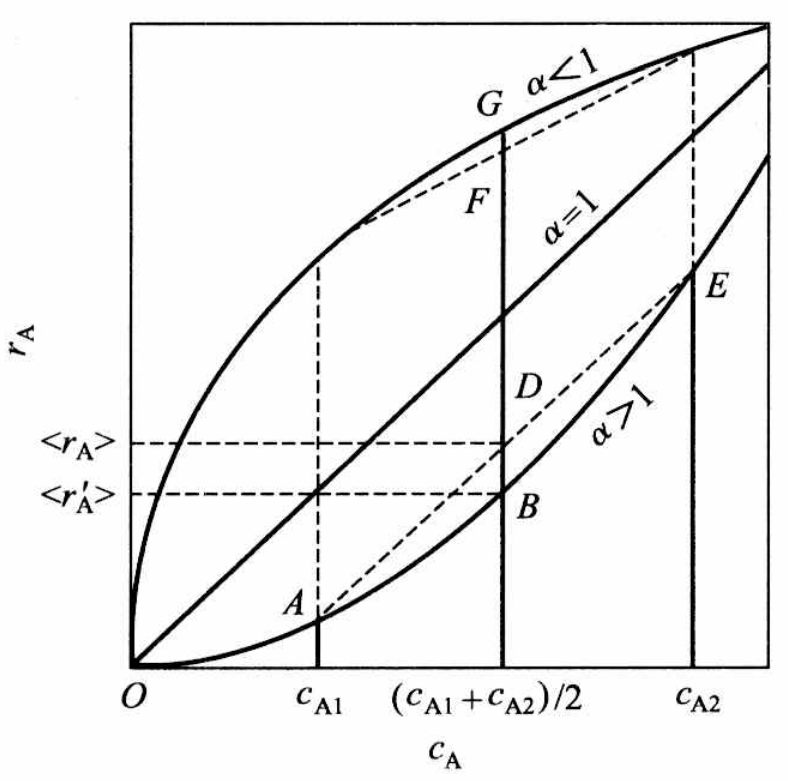
\includegraphics[width=\linewidth]{figures/fig5.25.png}
    \end{minipage}\hfill
    \begin{minipage}{0.48\linewidth}
        \begin{itemize}
            \item $\alpha=1$时，$\langle r_\mathrm{A}\rangle = \langle r_\mathrm{A}' \rangle$
            \item $\alpha>1$时，$\langle r_\mathrm{A}\rangle > \langle r_\mathrm{A}' \rangle$
            
            微观混合使平均反应速率下降。
            \item $\alpha<1$时，$\langle r_\mathrm{A}\rangle < \langle r_\mathrm{A}' \rangle$
            
            微观混合使平均反应速率加快。
        \end{itemize}
    \end{minipage}
    
\end{frame}


\begin{frame}
    \frametitle{微观混合对反应器工况的影响}

    \begin{itemize}
        \item 间歇反应器
        
        任何时刻下，间歇反应器中所有流体粒子均具有相同的停留时间，因而其组成亦应相同。所以微观混合的程度不影响反应器的工况。
        \item 活塞流反应器
        
        同一横截面上所有流体粒子停留时间相同，组成自然也相同，所以，微观混合的程度对活塞流反应器的工况不产生影响。
        \item 全混流反应器
        
        由于同一横截面上流体粒子的停留时间不同，其组成也就不同，于是，除一级反应外，微观混合的程度将影响反应器的工况。这种影响随着停留时间分布的不同而不同，返混程度越严重，微观混合程度的影响越大。
    \end{itemize}

\end{frame}


\begin{frame}
    \frametitle{微观混合对反应器工况的影响}

    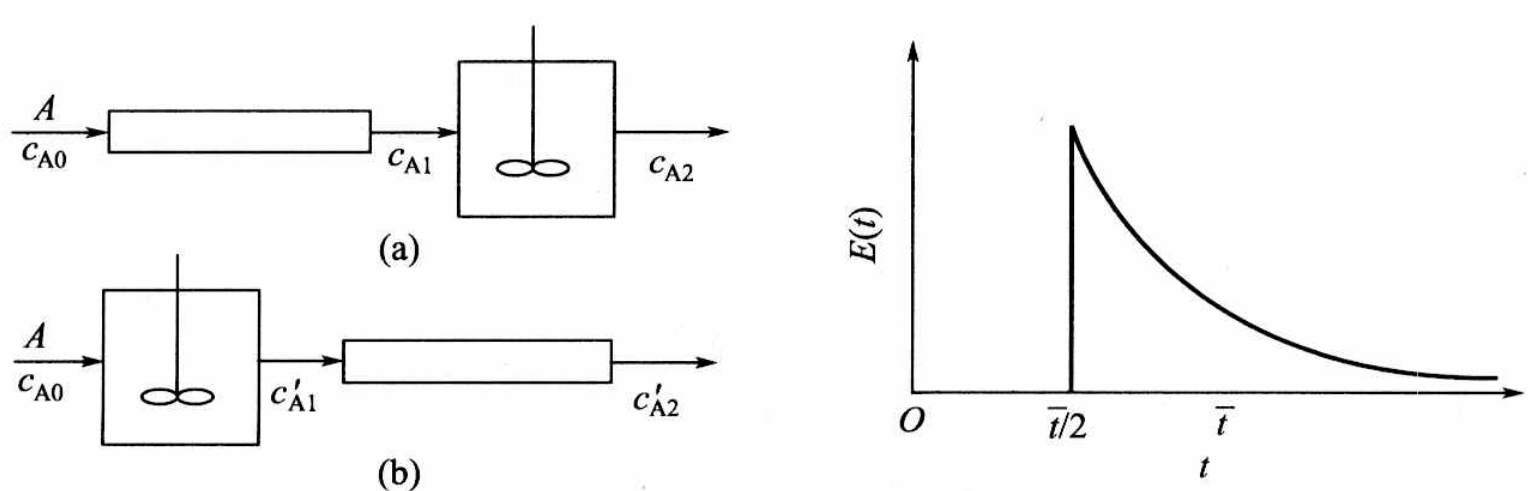
\includegraphics[width=\linewidth]{figures/fig5.26.png}

    (a) (b) 两种连接方式，停留时间分布相同，如果微观混合的程度也相同，是否两者的工况也相同呢？

\end{frame}


\begin{frame}[t]
    \frametitle{}

    \begin{example}
        如图所示两个串联反应器系统，在相同的温度及空时下进行同样的反应。若相串联的全混流反应器和活塞流反应器的空时均等于1 min，进口流体中$c_\mathrm{A0} = \SI{1}{kmol/m^3}$，试分别计算这两种串联情况所达到的转化率。假设所进行的反应为（1）一级反应；（2）二级反应，反应温度下两者的反应速率常数分别为\SI{1}{(min^{-1})}及\SI{1e-3}{m^3/(mol.min)}。        
    \end{example}
    \begin{figure}
        \centering
        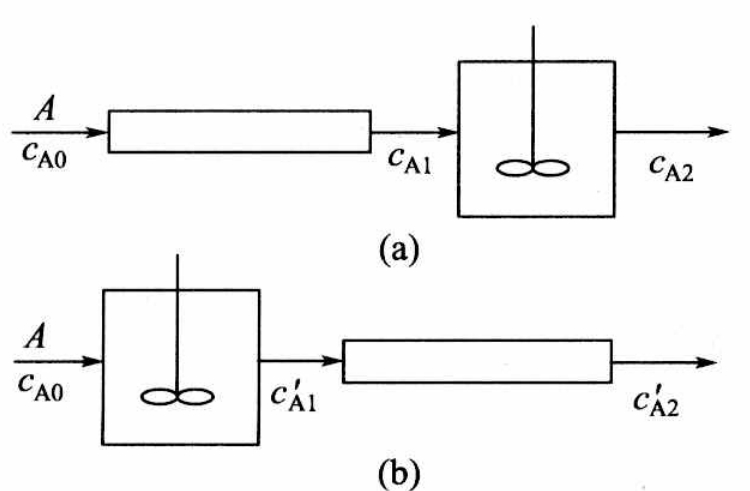
\includegraphics[width=.4\linewidth]{figures/fig5.26a.png}
    \end{figure}

\end{frame}

\end{document}